\documentclass[9pt]{beamer}

\usepackage{appendixnumberbeamer}
\usepackage{booktabs}
\usepackage[scale=2]{ccicons}
\usepackage{pgfplots}
\usepackage{tikz}
\usepackage{graphics}

\usepgfplotslibrary{dateplot}
\pdfstringdefDisableCommands{\def\translate#1{#1}}
\geometry{paperwidth=140mm, paperheight=105mm}
\usetheme{metropolis}
\bibliographystyle{abbrv}
\setbeamertemplate{frame footer}{Lab - Mechatronics}

\usetikzlibrary{shapes, arrows}
\tikzstyle{startstop} = [rectangle, rounded corners, minimum width=2cm, minimum height=1cm, text centered, draw=black, fill=red!30]
\tikzstyle{io} = [trapezium, trapezium stretches=true, trapezium left angle=70, trapezium right angle=110, minimum width=2cm, minimum height=1cm, text centered, draw=black, fill=blue!30]
\tikzstyle{process} = [rectangle, minimum width=2cm, minimum height=1cm, text centered, text width=2cm, draw=black, fill=orange!30]
\tikzstyle{decision} = [diamond, minimum width=2cm, minimum height=1cm, text centered, draw=black, fill=green!30]
\tikzstyle{arrow} = [thick,->,>=stealth]

\title{Modelling and control of a Magnetic Levitation System}
\subtitle{Mid-project presentation}
% \date{\today}
\date{November 07, 2024}
\author{Tommaso Bocchietti 10740309 \\ Daniele Cianca 10764733 \\ Sara Orazzo 10995845}
\institute{Politecnico di Milano}
\titlegraphic{\hfill
\includegraphics[height=1.5cm]{pdf/Polimi_logo_header.pdf}}

\begin{document}

\maketitle

\begin{frame}{Agenda}

    \begin{columns}[c, onlytextwidth]

        \begin{column}{0.4\textwidth}

            \setbeamertemplate{section in toc}[sections numbered]
            \tableofcontents

        \end{column}

        \begin{column}{0.6\textwidth}

            \begin{figure}[H]
                \centering
                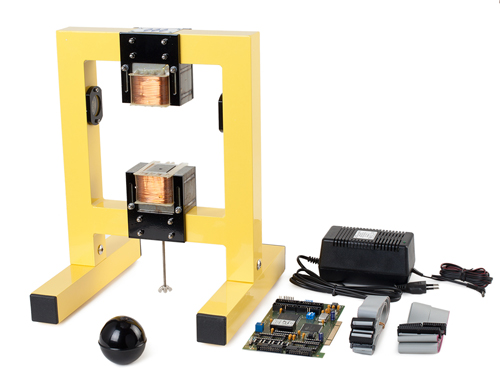
\includegraphics[width=0.8\textwidth]{img/maglev_and_components.jpg}
                \caption{Magnetic Levitation System and its components}
            \end{figure}

        \end{column}

    \end{columns}

\end{frame}

\begin{frame}{Project objectives}

    Magnetic Levitation System (MLS) it's an electromechanical system that enhances magnetic fields to levitate a ferromagnetic object.
    It's known for its non-linear behavior and its instability.

    \begin{columns}[c, onlytextwidth]

        \begin{column}{0.5\textwidth}

            \begin{figure}[H]
                \centering
                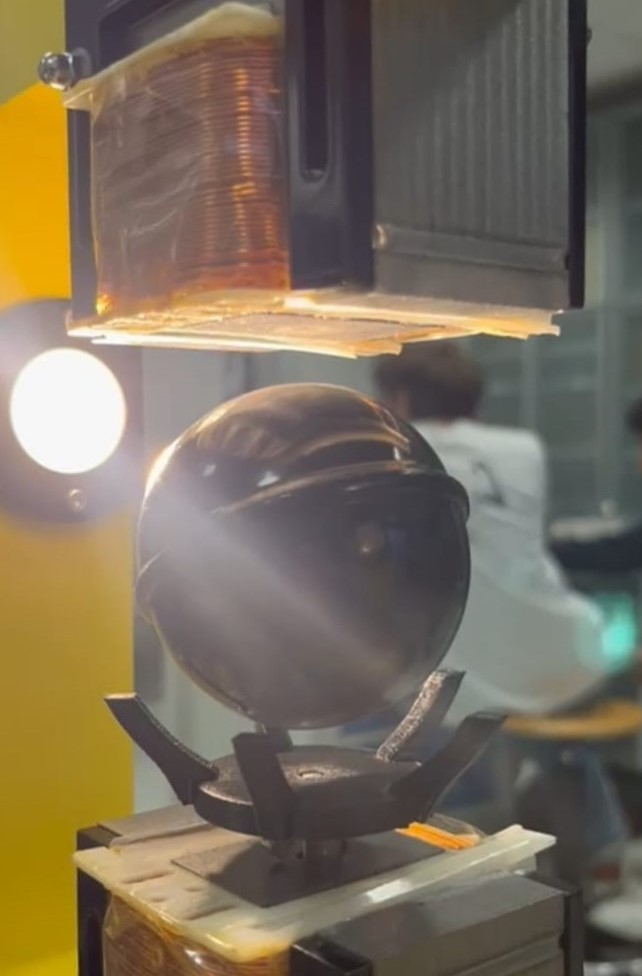
\includegraphics[width=0.7\textwidth]{img/ball_levitation.jpg}
            \end{figure}

        \end{column}

        \begin{column}{0.5\textwidth}

            \begin{center}
                Project objectives: \\
                \textbf{Make the ball levitate.}
            \end{center}

        \end{column}

    \end{columns}



\end{frame}
\section{What we have done}

\begin{frame}{Modelling}

    \only<1,2>{
        We derived the \textbf{equations of motion} of the Magnetic Levitation System (MLS) based on a Lagrangian approach.
    }

    \only<1>{


        \begin{equation}
            \frac{d}{dt} \left( \frac{\partial \mathcal{T}}{\partial \dot{\mathbf{u}}} \right) - \frac{\partial \mathcal{T}}{\partial \mathbf{u}} + \frac{\partial \mathcal{D}}{\partial \dot{\mathbf{u}}} + \frac{\partial \mathcal{U}}{\partial \mathbf{u}} = \mathcal{Q}
            \label{eq:lagrange_equation}
        \end{equation}

        \begin{equation}
            \begin{aligned}
                \mathcal{T} & = \frac{1}{2} m \dot{z}^2 + \frac{1}{2} L_1(z, \dot{q_1}, T_1) \dot{q_1}^2 + \frac{1}{2} L_2(z, \dot{q_2}, T_2) \dot{q_2}^2                                                                             \\
                \mathcal{D} & = \int_{\dot{z}(\cdot)} \frac{1}{2} C_d A \rho \dot{z}^2 d\dot{z} + \int_{\dot{q_1}(\cdot)} R_1(\dot{q_1}, T_1) \dot{q_1} d\dot{q_1} + \int_{\dot{q_2}(\cdot)} R_2(\dot{q_2}, T_2) \dot{q_2} d\dot{q_2} \\
                \mathcal{U} & = -m g z - q_1 V_1 - q_2 V_2                                                                                                                                                                            \\
                \mathcal{Q} & = 0
            \end{aligned}
        \end{equation}

    }

    \only<2>{
        \begin{equation}
            \begin{cases}
                m \ddot{z} - \frac{1}{2} \frac{\partial L_1}{\partial z} \dot{q_1}^2 - \frac{1}{2} \frac{\partial L_2}{\partial z} \dot{q_2}^2 + \frac{1}{2} C_d A \rho \dot{z} |\dot{z}| - m g = 0                                                                                                                                                                                                            \\
                \frac{1}{2} \left( \frac{\partial^2 L_1}{\partial \dot{q_1} \partial z} \dot{z} + \frac{\partial^2 L_1}{\partial \dot{q_1}^2} \ddot{q_1} \right) \dot{q_1}^2 + \frac{\partial L_1}{\partial \dot{q_1}} \dot{q_1} \ddot{q_1} + \left( \frac{\partial L_1}{\partial z} \dot{z} + \frac{\partial L_1}{\partial \dot{q_1}} \ddot{q_1} \right) \dot{q_1} + L_1 \ddot{q_1} + R_1 \dot{q_1} - V_1 = 0 \\
                \frac{1}{2} \left( \frac{\partial^2 L_2}{\partial \dot{q_2} \partial z} \dot{z} + \frac{\partial^2 L_2}{\partial \dot{q_2}^2} \ddot{q_2} \right) \dot{q_2}^2 + \frac{\partial L_2}{\partial \dot{q_2}} \dot{q_2} \ddot{q_2} + \left( \frac{\partial L_2}{\partial z} \dot{z} + \frac{\partial L_2}{\partial \dot{q_2}} \ddot{q_2} \right) \dot{q_2} + L_2 \ddot{q_2} + R_2 \dot{q_2} - V_2 = 0 \\
            \end{cases}
        \end{equation}
    }

    \only<3>{
        In order to simplify the model, we have \textbf{neglected the effect of the current on the value of the inductances (strong assumption)}.
        We also have neglected any velocity linearly dependent terms in the equations of motion.

        \begin{equation}
            \begin{cases}
                \frac{\partial L}{\partial I}     & \approx 0 \\
                \frac{\partial^2 L}{\partial I^2} & \approx 0 \\
                \dot{z}                           & \approx 0
            \end{cases}
            \label{eq:model_reduction_conditions}
        \end{equation}

        \vspace{9pt}

        From literature, we also have found an experimental based model for the inductances.

        \begin{equation}
            L = L(z) = L_0 + L_z e^{-a_z z}
        \end{equation}

    }

    \only<4>{
        The current model is a simplified version of the original one, but from experimental data we can see that it's still \textbf{able to capture the main dynamics of the system}.

        \begin{equation}
            \begin{cases}
                \dot{z} = v                                                                                                                                 \\
                \dot{v} = m^{-1} \left(\frac{1}{2} \frac{\partial L_1}{\partial z} I_1^2 + \frac{1}{2} \frac{\partial L_2}{\partial z} I_2^2 + m g  \right) \\
                \dot{I_1} = L_1^{-1} \left(- R_1 I_1 + (k_1 U_1 + c_1) \right)                                                                              \\
                \dot{I_2} = L_2^{-1} \left(- R_2 I_2 + (k_2 U_2 + c_2) \right)
            \end{cases}
            \label{eq:reduced_quations_of_motion_final}
        \end{equation}

        Notice that $z$ is the position of the ball (what we want to control), while $U_1$ and $U_2$ are the inputs of the system (what we can control).

    }

    \only<5>{
        The model has also been linearized and transformed in state-space form.

        \begin{equation}
            \begin{aligned}
                \dot{\mathbf{x}} & = f(\mathbf{x}, \mathbf{u}) \\
                \mathbf{y}       & = g(\mathbf{x}, \mathbf{u})
            \end{aligned}
            \quad
            \rightarrow
            \quad
            \begin{aligned}
                \dot{\delta\mathbf{x}} & \approx A \delta\mathbf{x} + B \delta\mathbf{u} \\
                \delta\mathbf{y}       & \approx C \delta\mathbf{x} + D \delta\mathbf{u}
            \end{aligned}
        \end{equation}

    }

\end{frame}



\begin{frame}{Parameters identification}

    \only<1>{
        In order to control the system, we had to \textbf{identify the parameters of the system}.
        To do so, many experiments have been conducted.
    }

    \only<2>{
        Control to Voltage mapping.

        \begin{columns}[c, onlytextwidth]

            \begin{column}{0.45\textwidth}

                As predictable, the control to voltage mapping is a linear function outside the `no control zone'.

                \begin{equation}
                    V = \begin{cases}
                        V_{min} & \text{if } U < U_{min}    \\
                        k U + c & \text{if } U \geq U_{min}
                    \end{cases}
                \end{equation}

            \end{column}

            \begin{column}{0.55\textwidth}

                \begin{figure}
                    \centering
                    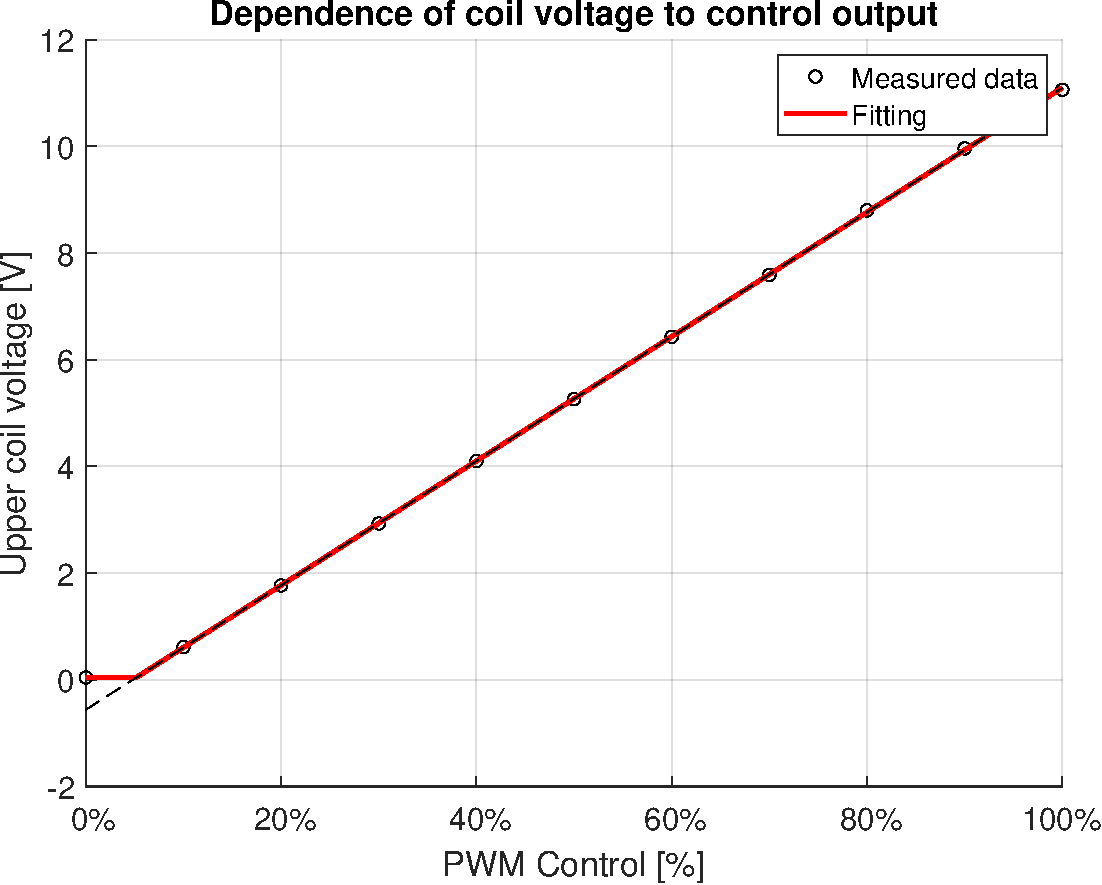
\includegraphics[width=0.8\textwidth]{img/MATLAB/measurements/control_to_voltage.pdf}
                    \caption{Voltage as a function of $U$}
                \end{figure}

            \end{column}

        \end{columns}

    }

    \only<3>{
        Electromagnetic force characterizations.

        \begin{columns}[c, onlytextwidth]

            \begin{column}{0.65\textwidth}

                \begin{figure}
                    \centering
                    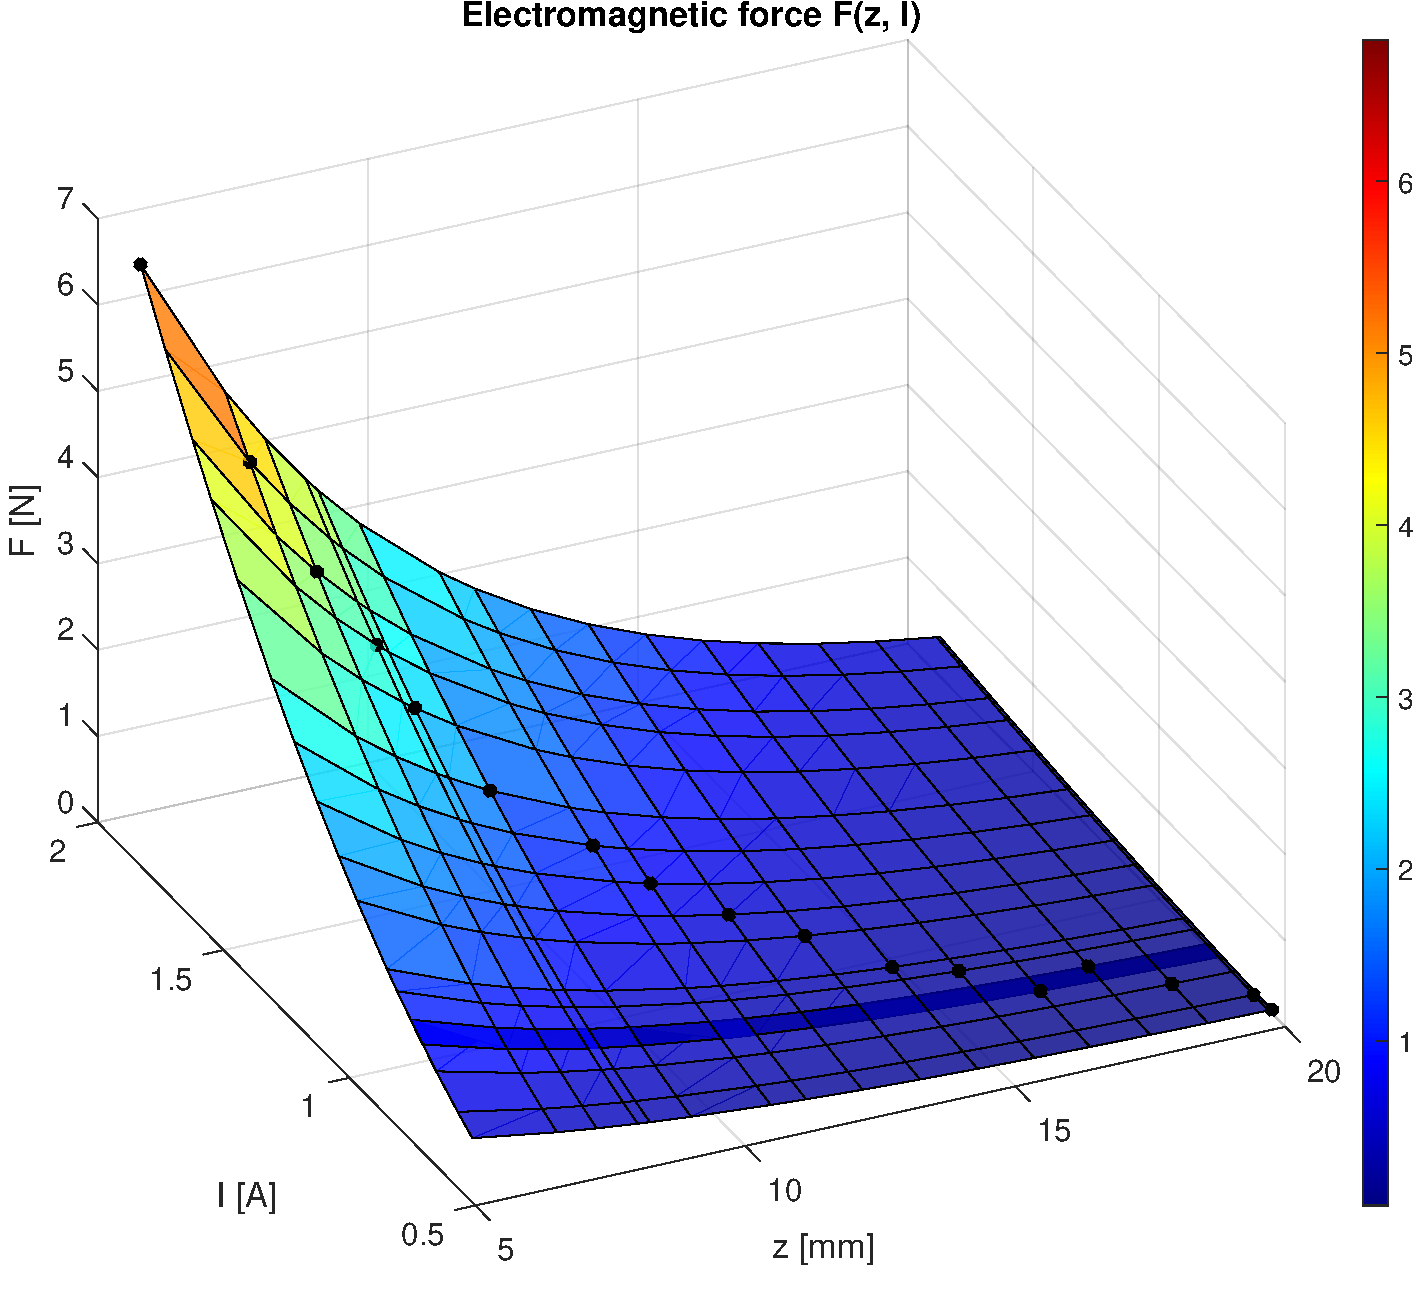
\includegraphics[width=0.8\textwidth]{img/MATLAB/measurements/force.pdf}
                    \caption{Electromagnetic force as a function of $z$ and $I$}
                \end{figure}

            \end{column}

            \begin{column}{0.35\textwidth}

                Notice that from the theoretical model, we have found the electromagnetic force acting on the ball to be:

                \begin{equation}
                    F_{em} = \frac{1}{2} \frac{\partial L}{\partial z} I^2
                \end{equation}

            \end{column}

        \end{columns}

    }

\end{frame}



\begin{frame}{Controlling}

    \only<1>{
        We have implemented a Simulink model of the system.

        \begin{figure}
            \centering
            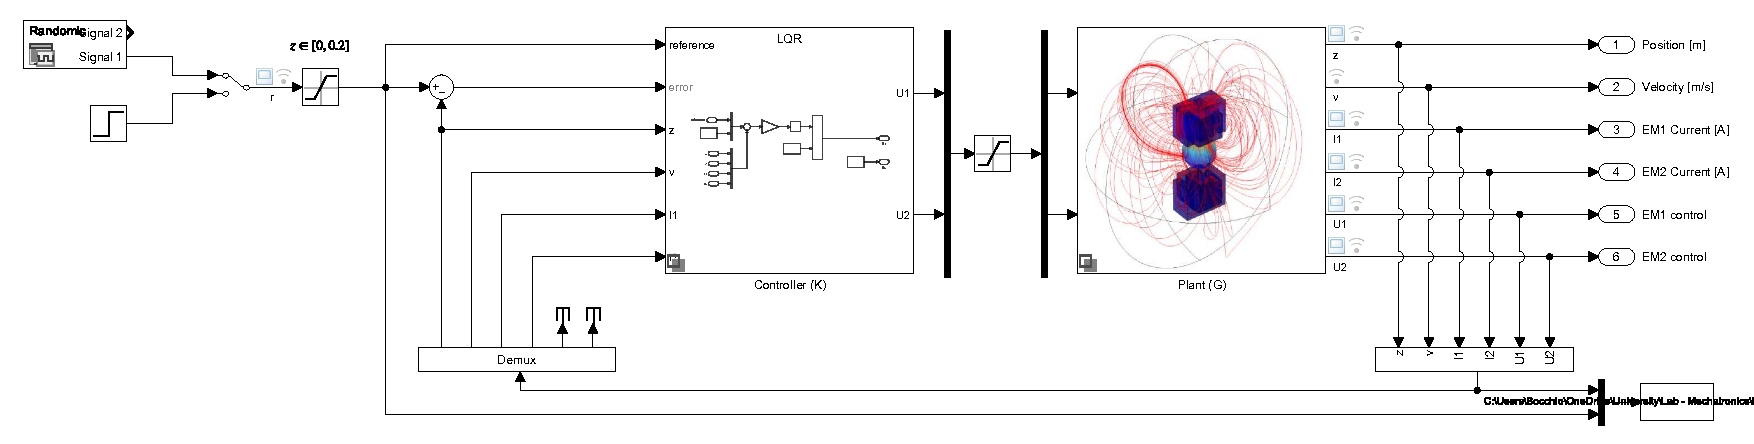
\includegraphics[width=1\textwidth]{img/MATLAB/simulink_model.pdf}
            \caption{Simulink root model of the Magnetic Levitation System}
        \end{figure}

        Some controllers have also been implemented and tested.

    }

    \only<2>{
        PID (both with and without anti-windup) controllers have been tested.

        \begin{figure}
            \centering
            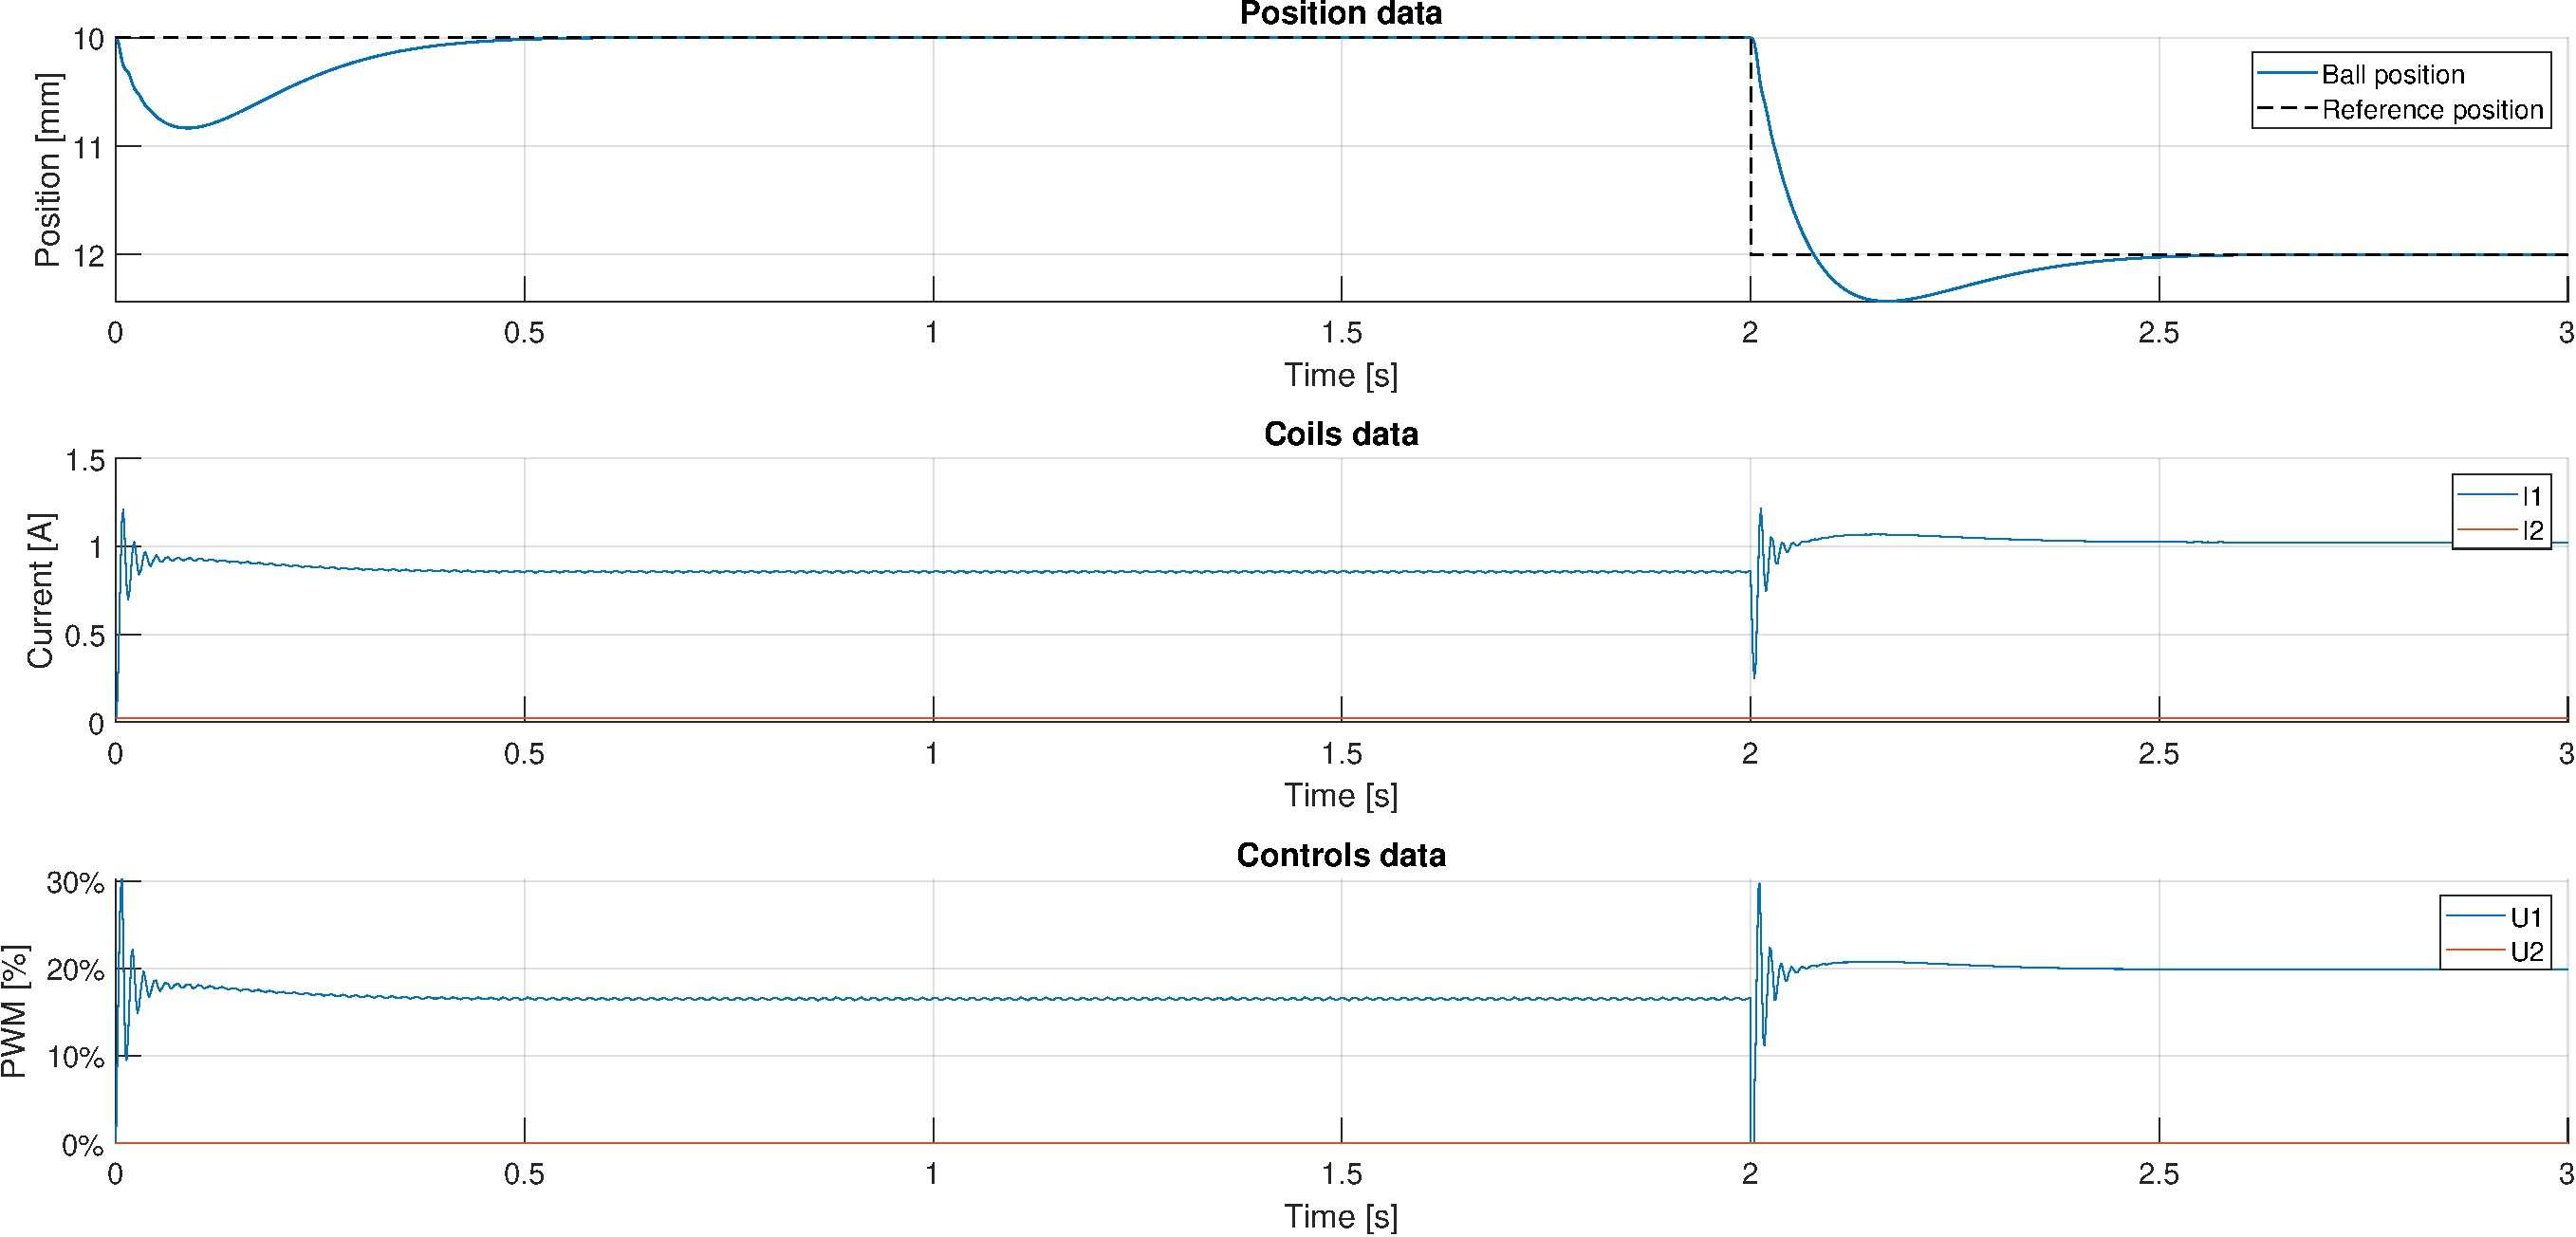
\includegraphics[width=1\textwidth]{img/MATLAB/runs/PID_anti_windup.pdf}
            \caption{PID with anti-windup controller}
        \end{figure}

        A PID controller without anti-windup has also been tested but with a clearly worse performance (strong oscillations around the reference).

    }

    \only<3>{
        LQR controllers with (limited) tracking capabilities have been tested.

        \begin{figure}
            \centering
            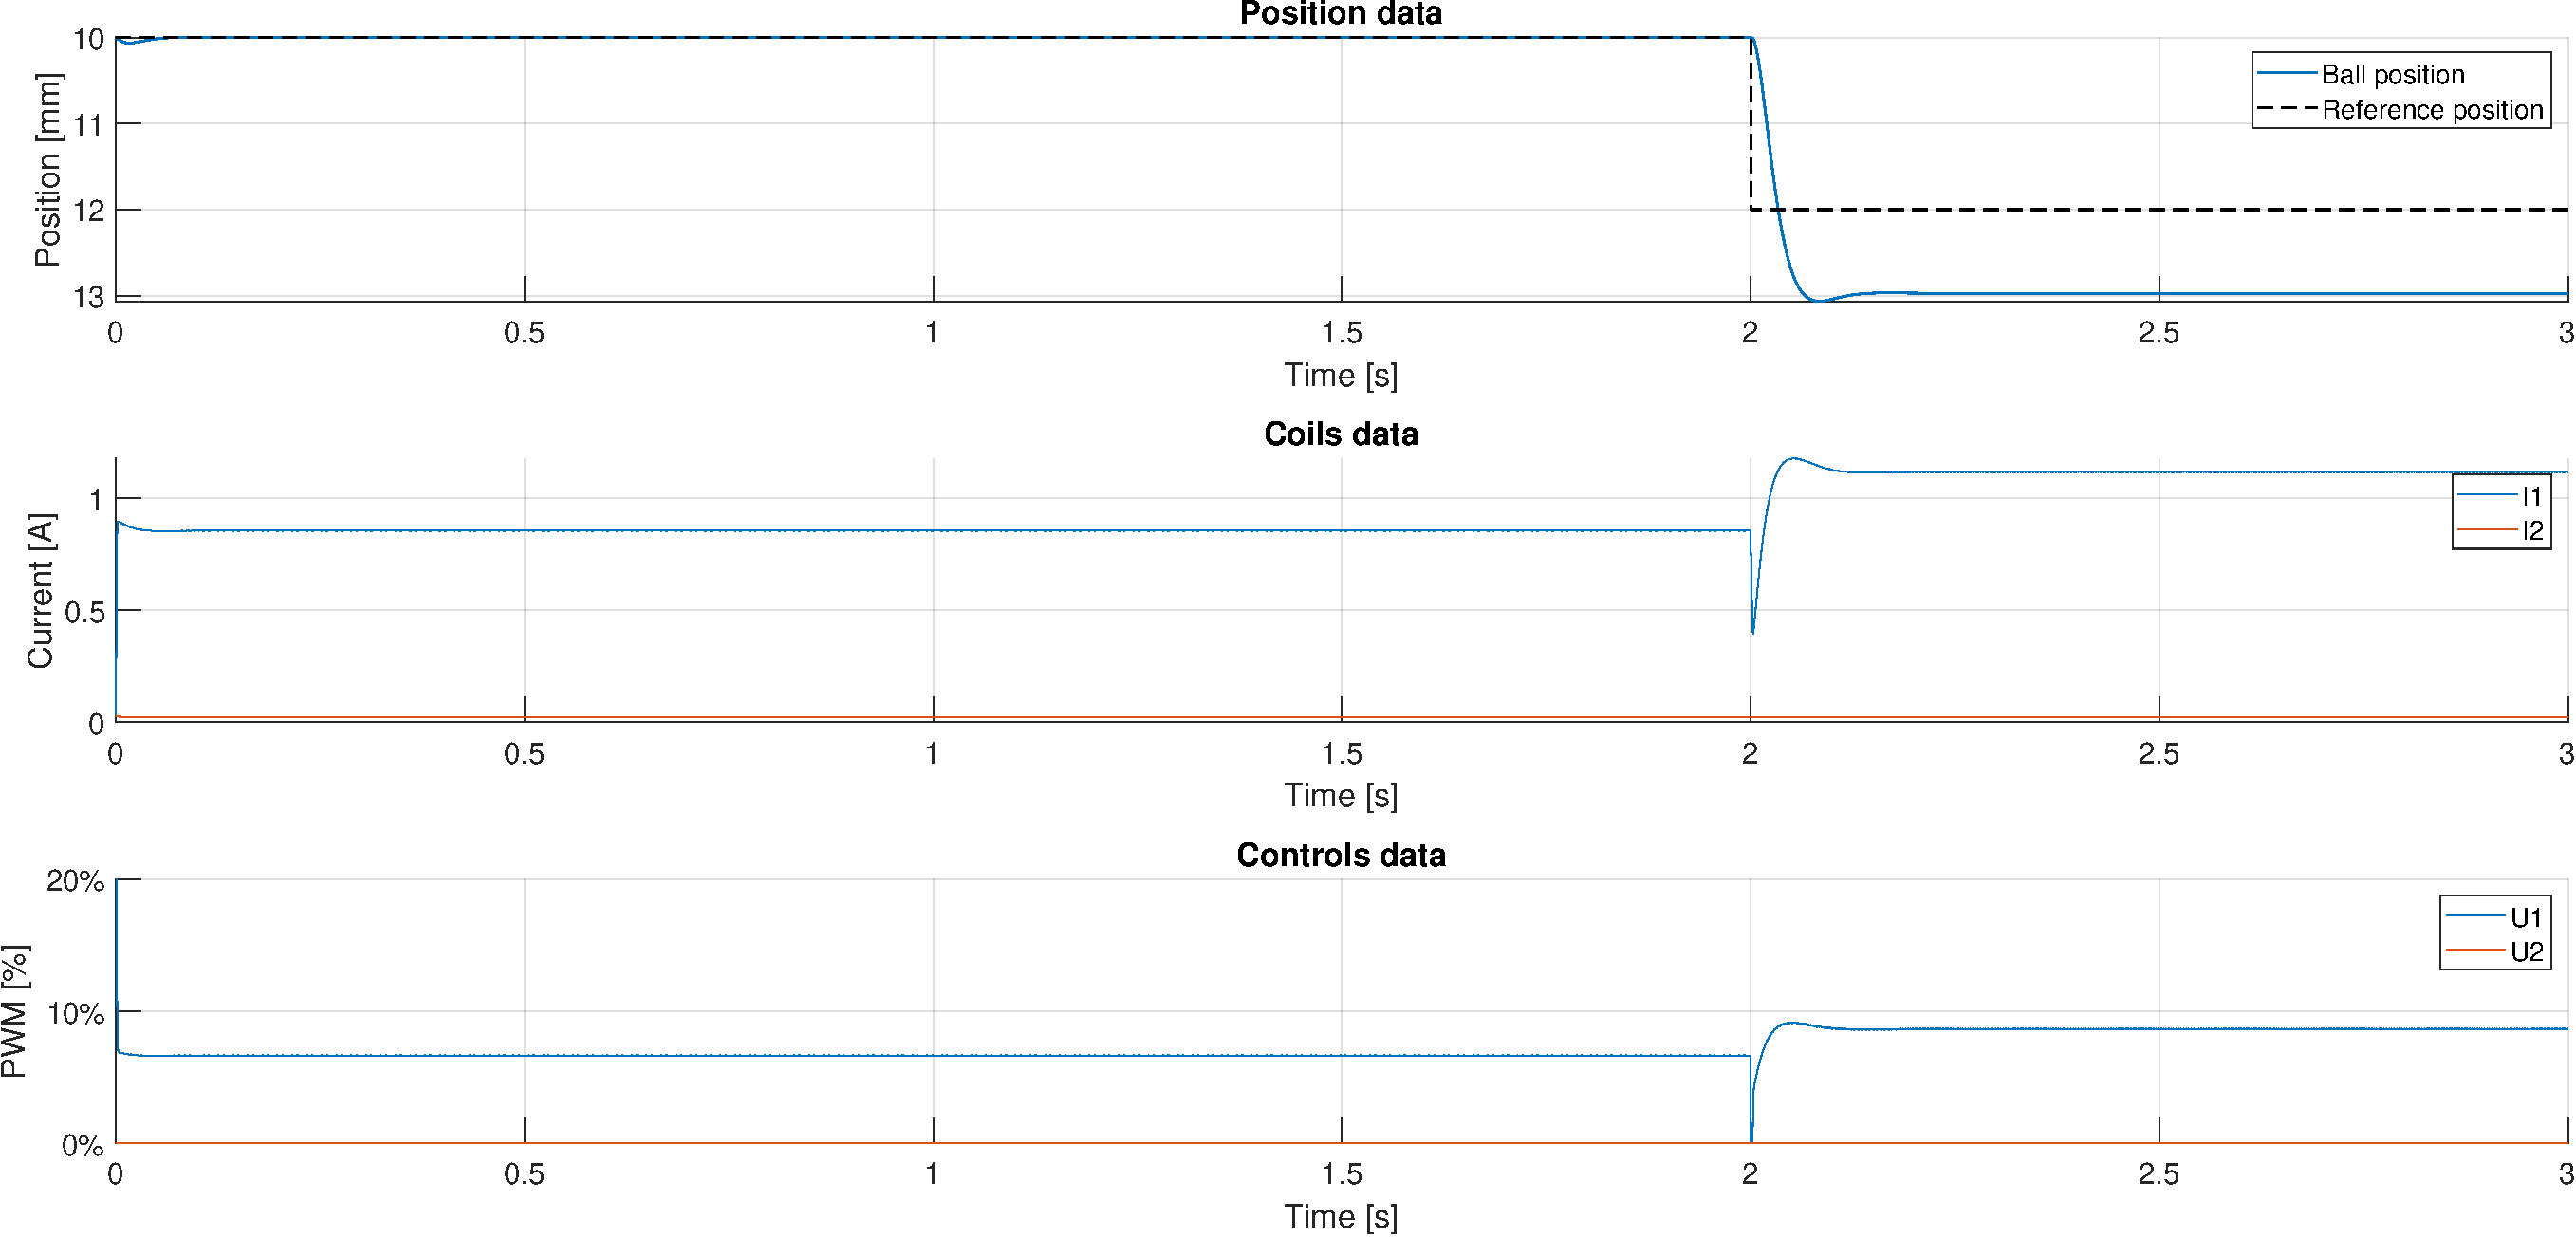
\includegraphics[width=1\textwidth]{img/MATLAB/runs/LQR_tracking.pdf}
            \caption{LQR controller}
        \end{figure}

    }

\end{frame}


\section{What we are working on}

\begin{frame}{Further inductance characterization}

    Even if maybe not relevant for control purposes, we are trying to \textbf{study the dependence of the inductance on both the ball position and the current}.
    \begin{equation}
        L = L(z, I) = L_0 + L_z e^{-a_z z} + L_I \tanh(-a_I I)
    \end{equation}

    \begin{columns}[c, onlytextwidth]

        \begin{column}{0.65\textwidth}

            \begin{figure}
                \centering
                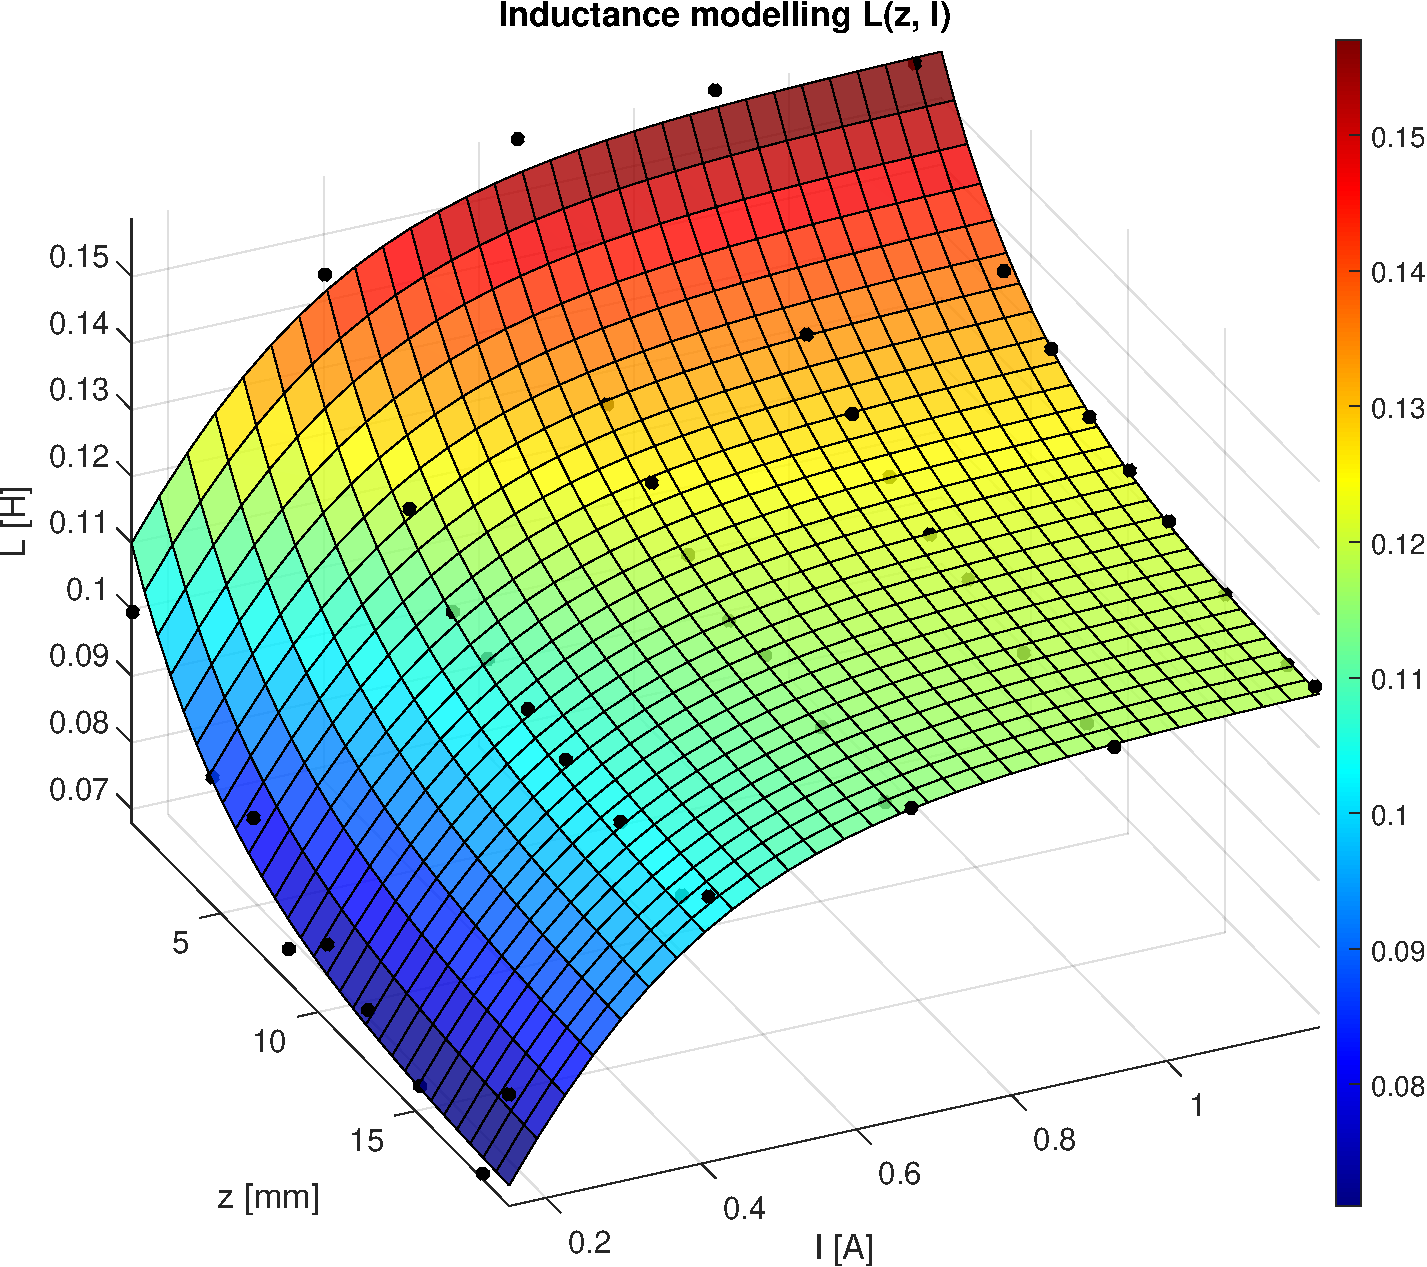
\includegraphics[width=0.8\textwidth]{img/MATLAB/measurements/inductance.pdf}
                \caption{Fitted model for $L(z, I)$}
            \end{figure}
        \end{column}

        \begin{column}{0.35\textwidth}

            Higher current values are needed to obtain experimental data over all the possible operating regions.

        \end{column}

    \end{columns}

\end{frame}



\begin{frame}{MCP controller}

    We are currently trying to implement a Model Predictive Controller (MPC).

    We want to switch from classical linearized restricted state-space controllers to a more advanced and robust controller.

    However, looks like Simulink doesn't really like the way we are doing it\dots many implementation issues.

\end{frame}
\section{What we would like to do}

\begin{frame}{Implement more advanced controllers}

    Nonlinear controllers are particularly interesting because of the highly nonlinear nature of the system.
    However, they look like they are going to be a challenge to implement.

    \vspace{9pt}

    \begin{columns}[T, onlytextwidth]

        \begin{column}{0.5\textwidth}

            \textbf{Linear Controllers}:

            \begin{itemize}
                \item Model Predictive Control
                \item Cascaded Control
                \item Pole Placement
                \item Linear Quadratic Integrator
            \end{itemize}

        \end{column}

        \begin{column}{0.5\textwidth}

            \textbf{Nonlinear Controllers}:

            \begin{itemize}
                \item Backstepping
                \item Feedback Linearization
            \end{itemize}

        \end{column}

    \end{columns}

    \vspace{9pt}

    When possible, we would also like to implement logics such as Kalman Filters or gain scheduling.

\end{frame}



\begin{frame}{Study the effects of approximations}

    Once the characterization of the inductances is complete, we would like to study the effects of the approximations we have made in the model.

    \vspace{9pt}

    For example by comparing:

    \begin{itemize}
        \item Linearized vs nonlinear model with respect to the real world system;
        \item Effects of simplified ($L(z)$) vs complete ($L(z, I)$) inductance modelling.
    \end{itemize}

\end{frame}



\begin{frame}{Controllers comparison}

    We would like to compare the performance of the controllers we have implemented.

    \vspace{9pt}

    To do so, we will probably create a `Race of Controllers\footnotemark[1]' where we will compare various performance indices.

    \footnotetext[1]{More on this in the final presentation.}

\end{frame}
\section{Open questions}

\begin{frame}{Questions}

    \begin{enumerate}
        \item \textbf{Influence of current on inductance}: is our assumption of neglecting the influence of current on inductance valid?
        \item \textbf{Use of a single coil}: implications and limitations of using a single vs double coil to control the system.
        \item \textbf{Discretization}: impact of discretization over controller's performance.
        \item \textbf{MPC linearization}: problems of linearization within the Model Predictive Control.
    \end{enumerate}

\end{frame}

\appendix

\begin{frame}[allowframebreaks]{References}
    \nocite{*}
    \bibliography{references}
\end{frame}

\begin{frame}[standout]
    Questions?
\end{frame}

\begin{frame}[standout]
    Thank you!
\end{frame}

\end{document}